% ============================================================
% Question Bank: ch04-06 Rewriting Expressions to Solve Problems
% Topic Title: Rewriting Expressions to Solve Problems
% CCSS: 7.EE.A.2
% Questions: 27 (15 MC + 6 SA + 6 Graphical)
% ============================================================

% --- Multiple Choice Questions (15) ---

\begin{practiceQuestion}{4-6-q01}{mc}
\begin{questionText}
A jacket costs $p$ dollars. The price increases by $15\%$. Which expression represents the new price?
\end{questionText}
\choiceA{$p + 15$}
\choiceB{$0.15p$}
\choiceC{$p + 0.15p = 1.15p$}
\choiceD{$15p$}
\correctAnswer{C}
\explanation{A $15\%$ increase means the new price is $p + 0.15p = (1 + 0.15)p = 1.15p$.}
\end{practiceQuestion}

\begin{practiceQuestion}{4-6-q02}{mc}
\begin{questionText}
A shirt originally costs $d$ dollars and is on sale for $30\%$ off. Which expression gives the sale price?
\end{questionText}
\choiceA{$d - 30$}
\choiceB{$0.30d$}
\choiceC{$d - 0.30d = 0.70d$}
\choiceD{$1.30d$}
\correctAnswer{C}
\explanation{$30\%$ off means you pay $100\% - 30\% = 70\%$ of the original. Sale price $= d - 0.30d = 0.70d$.}
\end{practiceQuestion}

\begin{practiceQuestion}{4-6-q03}{mc}
\begin{questionText}
A worker earns $w$ dollars per hour and gets a $12\%$ raise. Which expression represents the new hourly wage?
\end{questionText}
\choiceA{$w + 12$}
\choiceB{$1.12w$}
\choiceC{$0.12w$}
\choiceD{$w - 0.12w$}
\correctAnswer{B}
\explanation{$12\%$ raise: new wage $= w + 0.12w = 1.12w$.}
\end{practiceQuestion}

\begin{practiceQuestion}{4-6-q04}{mc}
\begin{questionText}
The expression $0.85m$ represents the cost of a membership after a discount. What percent discount was applied?
\end{questionText}
\choiceA{$85\%$}
\choiceB{$15\%$}
\choiceC{$0.85\%$}
\choiceD{$8.5\%$}
\correctAnswer{B}
\explanation{$0.85m = m - 0.15m$, which means $15\%$ was subtracted. The discount is $15\%$.}
\end{practiceQuestion}

\begin{practiceQuestion}{4-6-q05}{mc}
\begin{questionText}
The total cost of an item with $8\%$ sales tax is represented by which expression?
\end{questionText}
\choiceA{$c + 8$}
\choiceB{$0.08c$}
\choiceC{$c + 0.08c = 1.08c$}
\choiceD{$c - 0.08c$}
\correctAnswer{C}
\explanation{$8\%$ tax added to price $c$: total $= c + 0.08c = 1.08c$.}
\end{practiceQuestion}

\begin{practiceQuestion}{4-6-q06}{mc}
\begin{questionText}
Which expression is equivalent to $1.25s$?
\end{questionText}
\choiceA{$s + 25s$}
\choiceB{$s + 0.25s$}
\choiceC{$s - 0.25s$}
\choiceD{$s + 1.25$}
\correctAnswer{B}
\explanation{$1.25s = 1s + 0.25s = s + 0.25s$. This represents a $25\%$ increase of $s$.}
\end{practiceQuestion}

\begin{practiceQuestion}{4-6-q07}{mc}
\begin{questionText}
A store marks up its wholesale price by $40\%$. If the wholesale price is $h$ dollars, what is the retail price?
\end{questionText}
\choiceA{$h + 40$}
\choiceB{$0.40h$}
\choiceC{$1.40h$}
\choiceD{$h - 0.40h$}
\correctAnswer{C}
\explanation{Markup of $40\%$: retail $= h + 0.40h = 1.40h$.}
\end{practiceQuestion}

\begin{practiceQuestion}{4-6-q08}{mc}
\begin{questionText}
A car loses $18\%$ of its value each year. If the car is worth $v$ dollars now, what is its value after one year?
\end{questionText}
\choiceA{$v - 18$}
\choiceB{$0.18v$}
\choiceC{$0.82v$}
\choiceD{$1.18v$}
\correctAnswer{C}
\explanation{$18\%$ decrease: new value $= v - 0.18v = 0.82v$.}
\end{practiceQuestion}

\begin{practiceQuestion}{4-6-q09}{mc}
\begin{questionText}
The expression $1.065p$ represents a price after tax. What is the tax rate?
\end{questionText}
\choiceA{$1.065\%$}
\choiceB{$65\%$}
\choiceC{$10.65\%$}
\choiceD{$6.5\%$}
\correctAnswer{D}
\explanation{$1.065p = p + 0.065p$. The tax rate is $0.065 = 6.5\%$.}
\end{practiceQuestion}

\begin{practiceQuestion}{4-6-q10}{mc}
\begin{questionText}
A book costs $b$ dollars. First, a $10\%$ discount is applied, then $7\%$ tax is added. Which expression gives the final cost?
\end{questionText}
\choiceA{$1.07(0.90b)$}
\choiceB{$0.90(1.07b)$}
\choiceC{$b - 0.10b + 0.07b$}
\choiceD{Both A and B}
\correctAnswer{D}
\explanation{First apply discount: $0.90b$. Then add tax: $1.07(0.90b)$. Since multiplication is commutative, $0.90(1.07b)$ simplifies to the same final cost, so both A and B are correct.}
\end{practiceQuestion}

\begin{practiceQuestion}{4-6-q11}{mc}
\begin{questionText}
Maria says $0.75n$ means ``$75\%$ more than $n$.'' Is Maria correct?
\end{questionText}
\choiceA{Yes, $0.75n$ means $75\%$ more}
\choiceB{No, it means $25\%$ less than $n$}
\choiceC{No, it means $75\%$ of $n$, which is $25\%$ more}
\choiceD{Both B and C}
\correctAnswer{B}
\explanation{$0.75n = n - 0.25n$, so it represents $25\%$ less than $n$. Maria is incorrect because $0.75n$ is not $75\%$ more than $n$.}
\end{practiceQuestion}

\begin{practiceQuestion}{4-6-q12}{mc}
\begin{questionText}
A gym charges a monthly fee of $f$ dollars and increases it by $5\%$ each year. Which expression represents the fee after two annual increases?
\end{questionText}
\choiceA{$f + 0.10f$}
\choiceB{$1.05 \times 1.05 \times f$}
\choiceC{$f + 0.05f + 0.05f$}
\choiceD{$1.10f$}
\correctAnswer{B}
\explanation{After one year: $1.05f$. After two years: $1.05 \times 1.05f$. This is different from simply adding $10\%$ because each increase is on the already-increased amount.}
\end{practiceQuestion}

\begin{practiceQuestion}{4-6-q13}{mc}
\begin{questionText}
A farmer harvests $k$ bushels of corn. He sells $60\%$ at market and keeps the rest. How many bushels does he keep?
\end{questionText}
\choiceA{$k - 60$}
\choiceB{$0.60k$}
\choiceC{$0.40k$}
\choiceD{$1.60k$}
\correctAnswer{C}
\explanation{Sells $60\%$, keeps $100\% - 60\% = 40\%$. Amount kept $= 0.40k$.}
\end{practiceQuestion}

\begin{practiceQuestion}{4-6-q14}{mc}
\begin{questionText}
Two stores sell the same item at original price $r$. Store A offers $20\%$ off. Store B offers $10\%$ off, then another $10\%$ off the discounted price. Which store has a lower final price?
\end{questionText}
\choiceA{Store A is cheaper}
\choiceB{Store B is cheaper}
\choiceC{Both stores charge the same final price}
\choiceD{Cannot be determined without knowing $r$}
\correctAnswer{A}
\explanation{Store A: $0.80r$. Store B: $0.90(0.90r) = 0.81r$. Since $0.80r < 0.81r$, Store A is cheaper.}
\end{practiceQuestion}

\begin{practiceQuestion}{4-6-q15}{mc}
\begin{questionText}
Which situation can be represented by $0.92t$?
\end{questionText}
\choiceA{A $92\%$ tip added to a bill of $t$ dollars}
\choiceB{A $92\%$ increase in the number of tickets $t$}
\choiceC{An $8\%$ decrease in temperature $t$}
\choiceD{A $92\%$ decrease in time $t$}
\correctAnswer{C}
\explanation{$0.92t = t - 0.08t$, which represents an $8\%$ decrease from $t$.}
\end{practiceQuestion}

% --- Short Answer Questions (6) ---

\begin{practiceQuestion}{4-6-q16}{sa}
\begin{questionText}
Rewrite $n + 0.35n$ as a single term.
\end{questionText}
\correctAnswer{$1.35n$}
\explanation{$n + 0.35n = (1 + 0.35)n = 1.35n$. This represents a $35\%$ increase.}
\end{practiceQuestion}

\begin{practiceQuestion}{4-6-q17}{sa}
\begin{questionText}
A computer costs $c$ dollars. The price is reduced by $22\%$. Write the sale price as a single expression.
\end{questionText}
\correctAnswer{$0.78c$}
\explanation{$c - 0.22c = (1 - 0.22)c = 0.78c$.}
\end{practiceQuestion}

\begin{practiceQuestion}{4-6-q18}{sa}
\begin{questionText}
Explain what the expression $1.09x$ means in the context of a purchase where $x$ is the price before tax.
\end{questionText}
\correctAnswer{It represents the total cost after adding $9\%$ sales tax: $x + 0.09x = 1.09x$.}
\explanation{$1.09x = x + 0.09x$. The $0.09x$ is the $9\%$ tax, and $1.09x$ is the total with tax included.}
\end{practiceQuestion}

\begin{practiceQuestion}{4-6-q19}{sa}
\begin{questionText}
A $\$250$ bicycle is on sale for $15\%$ off. Then $6\%$ sales tax is added to the sale price. What is the final cost?
\end{questionText}
\correctAnswer{$\$225.25$}
\explanation{Sale price: $0.85 \times 250 = \$212.50$. Tax: $1.06 \times 212.50 = \$225.25$.}
\end{practiceQuestion}

\begin{practiceQuestion}{4-6-q20}{sa}
\begin{questionText}
Write $d - 0.45d$ as a single term and explain what percent of $d$ remains.
\end{questionText}
\correctAnswer{$0.55d$; $55\%$ of $d$ remains.}
\explanation{$d - 0.45d = (1 - 0.45)d = 0.55d$, which is $55\%$ of the original amount.}
\end{practiceQuestion}

\begin{practiceQuestion}{4-6-q21}{sa}
\begin{questionText}
A population of $p$ animals increases by $3\%$ one year and then decreases by $3\%$ the next year. Is the final population equal to $p$? Show your work.
\end{questionText}
\correctAnswer{No. After increase: $1.03p$. After decrease: $0.97(1.03p) = 0.9991p \neq p$, so the population is slightly less than $p$.}
\explanation{$1.03 \times 0.97 = 0.9991$. The final population is $0.9991p$, not $p$. Equal percent increase and decrease don't cancel out.}
\end{practiceQuestion}

% --- Graphical Multiple Choice Questions (3) ---

\begin{practiceQuestion}{4-6-q22}{gmc}
\begin{questionText}
The diagram shows two equivalent bars representing a price after a markup. Which expression represents the new price?

\begin{center}
\begin{tikzpicture}[scale=0.6]
  % Original bar
  \draw[thick, fill=funBlue!20] (0,2) rectangle (10,3.5);
  \node at (5,2.75) {Original price: $p$};
  % New bar with sections
  \draw[thick, fill=funBlue!20] (0,0) rectangle (10,1.5);
  \draw[thick, fill=funGreen!30] (10,0) rectangle (13,1.5);
  \node at (5,0.75) {$p$};
  \node at (11.5,0.75) {$0.30p$};
  \node[below] at (6.5,-0.3) {New price};
\end{tikzpicture}
\end{center}
\end{questionText}
\choiceA{$0.30p$}
\choiceB{$p + 30$}
\choiceC{$1.30p$}
\choiceD{$0.70p$}
\correctAnswer{C}
\explanation{New price $= p + 0.30p = 1.30p$. The diagram shows the original price plus a $30\%$ markup.}
\end{practiceQuestion}

\begin{practiceQuestion}{4-6-q23}{gmc}
\begin{questionText}
The table below shows equivalent expressions. Which value completes the table?

\begin{center}
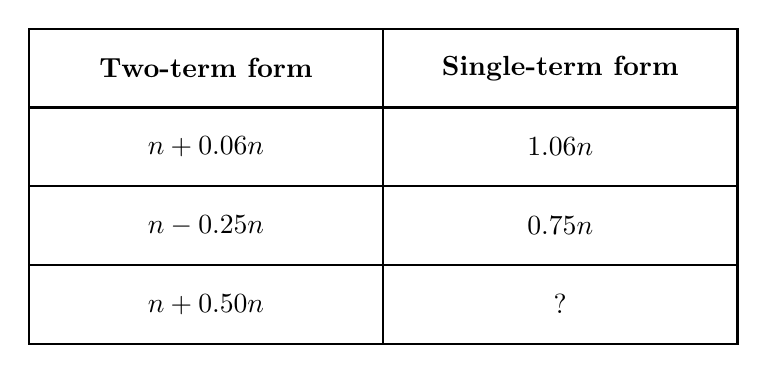
\begin{tikzpicture}
\draw[thick] (0,0) rectangle (9,4);
\draw[thick] (0,3) -- (9,3);
\draw[thick] (0,2) -- (9,2);
\draw[thick] (0,1) -- (9,1);
\draw[thick] (4.5,0) -- (4.5,4);
\node[font=\bfseries] at (2.25,3.5) {Two-term form};
\node[font=\bfseries] at (6.75,3.5) {Single-term form};
\node at (2.25,2.5) {$n + 0.06n$};
\node at (6.75,2.5) {$1.06n$};
\node at (2.25,1.5) {$n - 0.25n$};
\node at (6.75,1.5) {$0.75n$};
\node at (2.25,0.5) {$n + 0.50n$};
\node at (6.75,0.5) {?};
\end{tikzpicture}
\end{center}
\end{questionText}
\choiceA{$0.50n$}
\choiceB{$1.50n$}
\choiceC{$1.05n$}
\choiceD{$50n$}
\correctAnswer{B}
\explanation{$n + 0.50n = (1 + 0.50)n = 1.50n$.}
\end{practiceQuestion}

\begin{practiceQuestion}{4-6-q24}{gmc}
\begin{questionText}
The flow chart below shows steps applied to a price. What single multiplier achieves the same result?

\begin{center}
\begin{tikzpicture}[scale=0.7, node distance=2.5cm]
  \node[draw, thick, rounded corners, fill=funBlue!15, minimum width=2cm, minimum height=0.8cm] (start) {Price: $x$};
  \node[draw, thick, rounded corners, fill=funOrange!15, minimum width=2.8cm, minimum height=0.8cm, right of=start, xshift=1.5cm] (step1) {Discount $25\%$};
  \node[draw, thick, rounded corners, fill=funGreen!15, minimum width=2.2cm, minimum height=0.8cm, right of=step1, xshift=1.5cm] (step2) {Add $10\%$ tax};
  \node[draw, thick, rounded corners, fill=funBlue!15, minimum width=2cm, minimum height=0.8cm, right of=step2, xshift=1.5cm] (end) {Final: $?$};
  \draw[->, thick] (start) -- (step1);
  \draw[->, thick] (step1) -- (step2);
  \draw[->, thick] (step2) -- (end);
\end{tikzpicture}
\end{center}
\end{questionText}
\choiceA{$0.825x$}
\choiceB{$0.85x$}
\choiceC{$0.65x$}
\choiceD{$1.35x$}
\correctAnswer{A}
\explanation{Discount $25\%$: $0.75x$. Add $10\%$ tax: $1.10(0.75x) = 0.825x$.}
\end{practiceQuestion}

% --- Graphical Short Answer Questions (3) ---

\begin{practiceQuestion}{4-6-q25}{gsa}
\begin{questionText}
The double number line below shows the relationship between a percentage and a price. Fill in the missing value marked with $?$.

\begin{center}
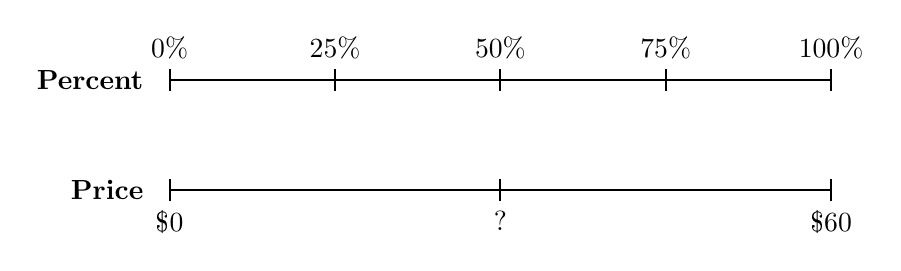
\begin{tikzpicture}[scale=0.7]
  % Top line (percent)
  \draw[thick] (0,2) -- (12,2);
  \foreach \x/\label in {0/0\%, 3/25\%, 6/50\%, 9/75\%, 12/100\%} {
    \draw[thick] (\x,1.8) -- (\x,2.2);
    \node[above] at (\x,2.2) {\label};
  }
  % Bottom line (price)
  \draw[thick] (0,0) -- (12,0);
  \foreach \x/\label in {0/\$0, 6/?, 12/\$60} {
    \draw[thick] (\x,-0.2) -- (\x,0.2);
    \node[below] at (\x,-0.2) {\label};
  }
  \node[left] at (-0.3,2) {\textbf{Percent}};
  \node[left] at (-0.3,0) {\textbf{Price}};
\end{tikzpicture}
\end{center}
\end{questionText}
\correctAnswer{$\$30$}
\explanation{$50\%$ of $\$60$ is $0.50 \times 60 = \$30$.}
\end{practiceQuestion}

\begin{practiceQuestion}{4-6-q26}{gsa}
\begin{questionText}
The receipt below shows a purchase. Calculate the total after tax and explain using expressions.

\begin{center}
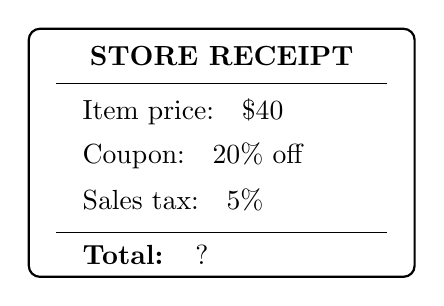
\begin{tikzpicture}[scale=0.7]
  \draw[thick, rounded corners] (0,0) rectangle (7,4.5);
  \node[font=\bfseries] at (3.5,4) {STORE RECEIPT};
  \draw (0.5,3.5) -- (6.5,3.5);
  \node[anchor=west] at (0.8,3) {Item price:\quad $\$40$};
  \node[anchor=west] at (0.8,2.2) {Coupon:\quad $20\%$ off};
  \node[anchor=west] at (0.8,1.4) {Sales tax:\quad $5\%$};
  \draw (0.5,0.8) -- (6.5,0.8);
  \node[anchor=west, font=\bfseries] at (0.8,0.4) {Total:\quad $?$};
\end{tikzpicture}
\end{center}
\end{questionText}
\correctAnswer{$\$33.60$}
\explanation{After coupon: $0.80 \times 40 = \$32$. After tax: $1.05 \times 32 = \$33.60$. Expression: $1.05(0.80 \times 40) = 1.05(32) = 33.60$.}
\end{practiceQuestion}

\begin{practiceQuestion}{4-6-q27}{gsa}
\begin{questionText}
The graph compares two plans for growing a savings account of $s$ dollars over one year. Plan A increases by $20\%$ once. Plan B increases by $10\%$ twice (every 6 months). Write the expression for each plan's final amount and determine which plan gives more money.

\begin{center}
\begin{tikzpicture}[scale=0.7]
  % Plan A
  \node[draw, thick, rounded corners, fill=funBlue!15, minimum width=3cm, minimum height=1cm] (a1) at (0,3) {Start: $s$};
  \node[draw, thick, rounded corners, fill=funBlue!30, minimum width=3cm, minimum height=1cm] (a2) at (6,3) {End: $?$};
  \draw[->, thick] (a1) -- node[above] {$+20\%$} (a2);
  \node[left] at (-1.8,3) {\textbf{Plan A}};
  % Plan B
  \node[draw, thick, rounded corners, fill=funGreen!15, minimum width=3cm, minimum height=1cm] (b1) at (0,0) {Start: $s$};
  \node[draw, thick, rounded corners, fill=funGreen!25, minimum width=3cm, minimum height=1cm] (b2) at (4.5,0) {$6$ mo: $?$};
  \node[draw, thick, rounded corners, fill=funGreen!35, minimum width=3cm, minimum height=1cm] (b3) at (9.5,0) {End: $?$};
  \draw[->, thick] (b1) -- node[above] {$+10\%$} (b2);
  \draw[->, thick] (b2) -- node[above] {$+10\%$} (b3);
  \node[left] at (-1.8,0) {\textbf{Plan B}};
\end{tikzpicture}
\end{center}
\end{questionText}
\correctAnswer{Plan A: $1.20s$. Plan B: $1.10 \times 1.10s = 1.21s$. Plan B gives more money.}
\explanation{Plan A: $s + 0.20s = 1.20s$. Plan B: $1.10(1.10s) = 1.21s$. Since $1.21s > 1.20s$, Plan B yields more. Two $10\%$ increases compound to more than a single $20\%$ increase.}
\end{practiceQuestion}
